\documentclass[a4paper,10pt]{article}
\usepackage[utf8]{inputenc}
\usepackage{amsmath}
\usepackage{fullpage}
\usepackage{hyperref}
\usepackage{graphicx}
\usepackage{listings}
\usepackage{color}

\definecolor{mygreen}{rgb}{0,0.6,0}
\definecolor{mygray}{rgb}{0.5,0.5,0.5}
\definecolor{mymauve}{rgb}{0.58,0,0.82}

\lstset{ 
  backgroundcolor=\color{white},   % choose the background color; you must add \usepackage{color} or \usepackage{xcolor}; should come as last argument
  basicstyle=\footnotesize,        % the size of the fonts that are used for the code
  breakatwhitespace=false,         % sets if automatic breaks should only happen at whitespace
  breaklines=true,                 % sets automatic line breaking
  captionpos=b,                    % sets the caption-position to bottom
  commentstyle=\color{mygreen},    % comment style
  deletekeywords={...},            % if you want to delete keywords from the given language
  escapeinside={\%*}{*)},          % if you want to add LaTeX within your code
  extendedchars=true,              % lets you use non-ASCII characters; for 8-bits encodings only, does not work with UTF-8
  firstnumber=1,                   % start line enumeration with line 1000
  frame=single,	                   % adds a frame around the code
  keepspaces=true,                 % keeps spaces in text, useful for keeping indentation of code (possibly needs columns=flexible)
  keywordstyle=\color{blue},       % keyword style
  language=Python,                 % the language of the code
  morekeywords={*,...},            % if you want to add more keywords to the set
  numbers=left,                    % where to put the line-numbers; possible values are (none, left, right)
  numbersep=5pt,                   % how far the line-numbers are from the code
  numberstyle=\tiny\color{mygray}, % the style that is used for the line-numbers
  rulecolor=\color{black},         % if not set, the frame-color may be changed on line-breaks within not-black text (e.g. comments (green here))
  showspaces=false,                % show spaces everywhere adding particular underscores; it overrides 'showstringspaces'
  showstringspaces=false,          % underline spaces within strings only
  showtabs=false,                  % show tabs within strings adding particular underscores
  stepnumber=1,                    % the step between two line-numbers. If it's 1, each line will be numbered
  stringstyle=\color{mymauve},     % string literal style
  tabsize=4,	                   % sets default tabsize to 2 spaces
  title=\lstname                   % show the filename of files included with \lstinputlisting; also try caption instead of title
}


%opening
\title{NUR Assignment 2}
\author{Christiaan van Buchem - s1587064}

\begin{document}

\maketitle

\begin{abstract}
 In this document I will be giving my answers to the questions of the second assignment for the Numerical Recipes for Astrophysics course. For each question I will give a short introduction, write out any non-coded answers that may be required, produce the print statements and the plots, and finally I will show the script used to produce the results.  
\end{abstract}

\section{Normally distributed pseudo-random numbers}

\subsection{RNG}

For exercise 1 we were tasked with writing a random number generator that returns a random floating point number between 0 and 1. At minimum we had to use some combination of an MWC and a 64-bit XOR-shift. The plots made to test the quality of the RNG can be seen in Figures \ref{fig:1a}, \ref{fig:1b}, and \ref{fig:1c}.


\begin{figure}[h!] 
	\begin{center}
    	%
		\subfigure{%
			\label{fig:1a}
			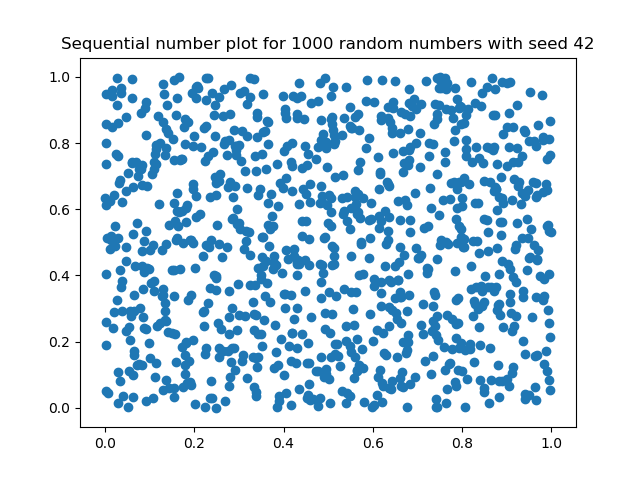
\includegraphics[width=0.45\linewidth]{./plots/1a.png}
		}%
		\subfigure{%
			\label{fig:1b}
			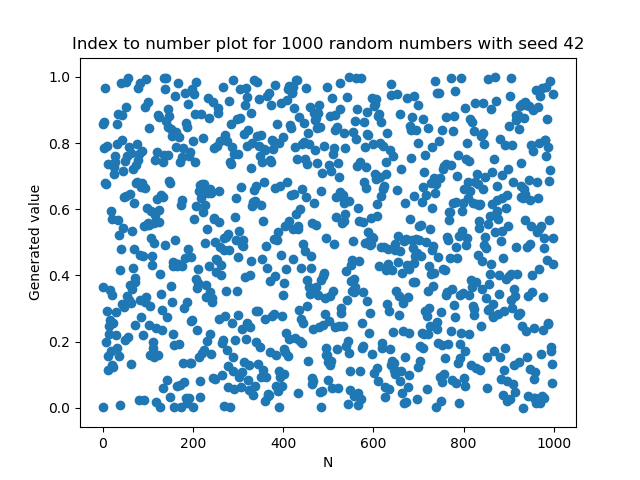
\includegraphics[width=0.45\linewidth]{./plots/1b.png}
		}
	\end{center}
	\captionsetup{width=0.8\linewidth}
	\vspace*{-7mm} %reduce space between caption and figure
	\caption{\textit{Left:} Sequential number plot showing that it appears that each number is independent of its predecessor. \textit{Right:} Index to number plot showing that there does not appear to be a relation between the index of a number and its value.}
	\label{fig:1ab}
\end{figure}

\begin{figure}[h!]
  \centering
  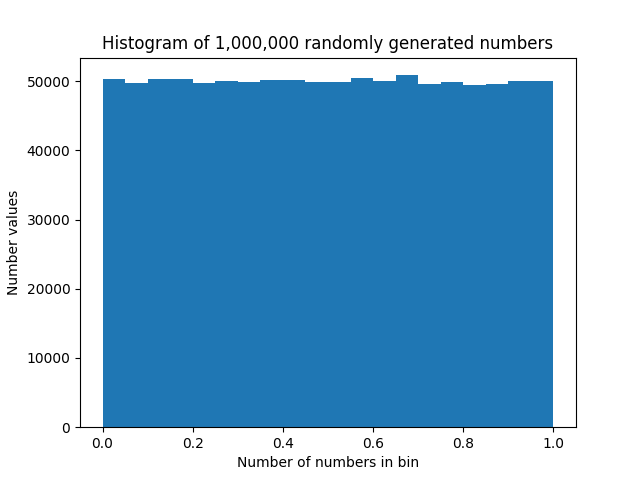
\includegraphics[width=0.8\linewidth]{./plots/1c.png}
  \caption{This histogram places the random number generator under a sharper knife, allowing us to see that there are some fluctuations between the bins. Overal it appears to be quite unbiased.}
  \label{fig:1c}
\end{figure}

\subsection{Box-Muller method}
Using the Box-Muller method we had to generate 1000 normally distributed random numbers. In order to check if they follow the expected distribution we make a histogram with an over-plotted Gaussian. The results can be seen in Figure \ref{fig:1d}.

\begin{figure}[h!]
  \centering
  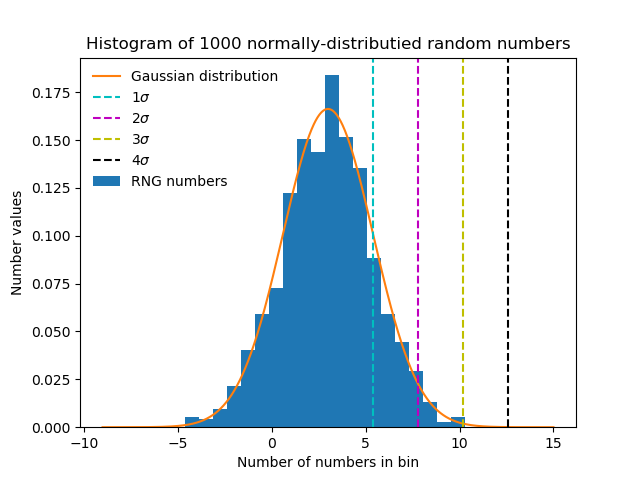
\includegraphics[width=0.8\linewidth]{./plots/1d.png}
  \caption{In this figure we can see that numbers generated using the Box-Muller method do indeed follow the Gaussian distribution.}
  \label{fig:1d}
\end{figure}

\subsection{KS-test}
For this exercise we tested whether or not our function is consistent with the normal distribution. The resulting plot can be seen in Figure \ref{fig:1e}. The slight difference between the two may be attributed to the fact that in the self written KS-test the following approximation was used: 
\[
	P_{KS}(z)\approx
\begin{cases}
	\frac{\sqrt{2\pi}}{z}[(e^{-\pi^2/(8z^2)})+(e^{-\pi^2/(8z^2)})^9+(e^{-\pi^2/(8z^2)})^25],& (z<1.18)\\
	1-2[(e^{-2z^2})-(e^{-2z^2})^4+(e^{-2z^2})^9],	& (z\geq 1.18)
\end{cases}
\]


\begin{figure}[h!]
  \centering
  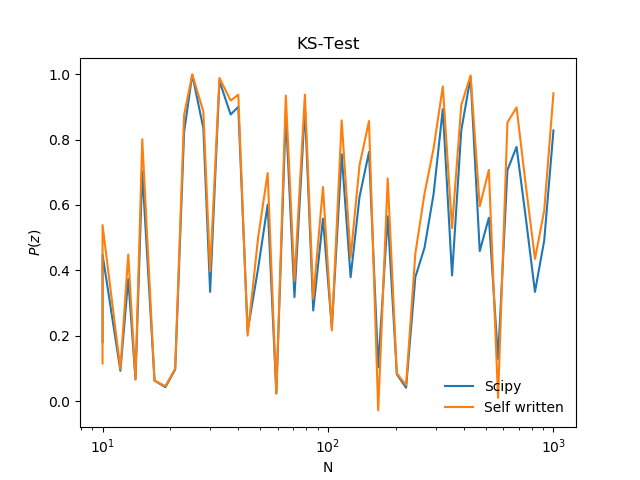
\includegraphics[width=0.8\linewidth]{./plots/1e.png}
  \caption{Here we see that the 'self-written' KS-test follows the Scipy KS-test results almost exactly.}
  \label{fig:1e}
\end{figure}

\subsection{Kuiper's-test}

The same as for the KS-test except that we had to use Kuiper's test. Results can be seen in Figure \ref{fig:1f}.

\begin{figure}[h!]
  \centering
  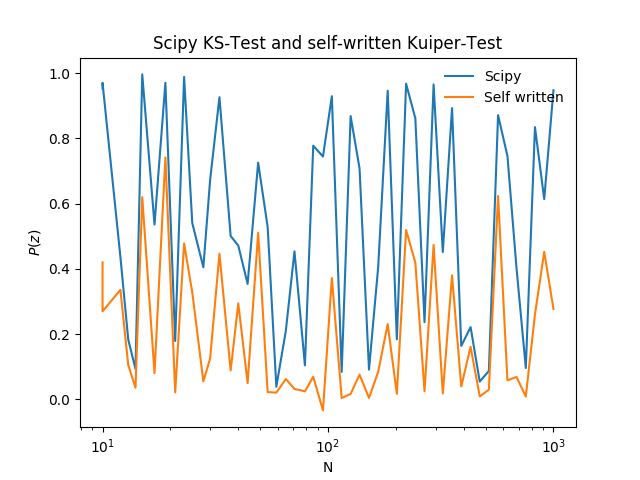
\includegraphics[width=0.8\linewidth]{./plots/1f.png}
  \caption{Here we compare the Kuipers test.}
  \label{fig:1f}
\end{figure}

\subsection{Analysing a dataset}

In this exercise we were tasked with analysing a giving data set using either the KS-test or Kuipers test. The results can be seen in Figure \ref{fig:1g}. We decided to use the KS-Test for this exercise. It appears that the 3rd data set has also been drawn from a normal distribution due to the fact that it is the only one that remains above 0.

\begin{figure}[h!]
  \centering
  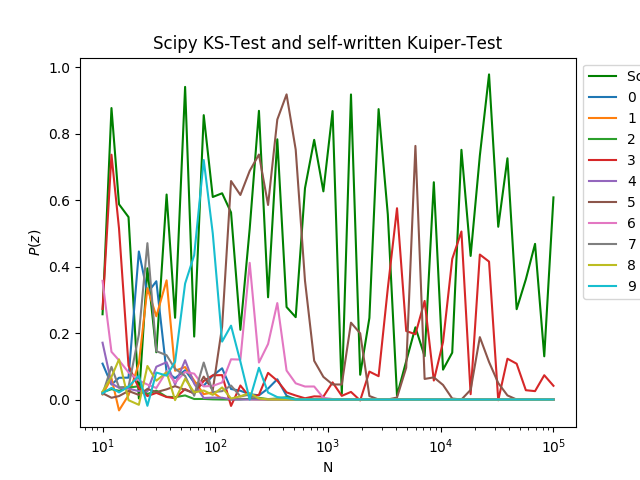
\includegraphics[width=0.8\linewidth]{./plots/1g.png}
  \caption{Analysing the different datasets.}
  \label{fig:1g}
\end{figure}

\subsection{Scripts}

Here we can see the terminal output of the script used for this exercise:
\lstinputlisting{a2_1.txt}

Here is the script used to produce these results: 
\lstinputlisting{a2_1.py}

\section{Making an initial density field}

For this exercise we were asked to generate a Gaussian random field. The field is generated in Fourier Space. The complex Fourier amplitudes are given by $\tilde{Y}=|\tilde{Y}exp(i\phi)$ where $phi$ is a random phase. The power spectrum has the following form: 

\begin{equation}
P(k) \propto k^n
\end{equation}

In Figure \ref{fig:2} the generated Gaussian random fields are given for different n values. 

\color{red}
Choose a minimum physical size and explain how this impacts the maximum physical size, the minimum $k$ and maximum $k$. 

\color{black}

\begin{figure}[h!]
  \centering
  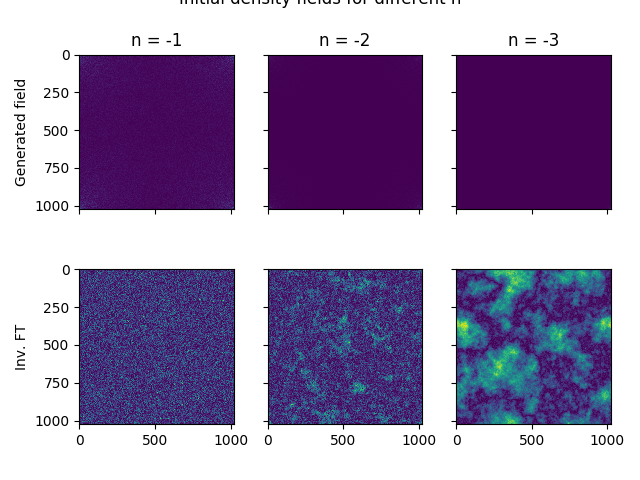
\includegraphics[width=0.8\linewidth]{./plots/2.png}
  \caption{Gaussian random fields for different n values. Notice the clear presence of larger structure when the spectrum is more peaked (lower n).}
  \label{fig:2}
\end{figure}

\subsection{Scripts}

Here we can see the terminal output of the script used for this exercise:
\lstinputlisting{a2_2.txt}

Here is the script used to produce these results: 
\lstinputlisting{a2_2.py}

\section{Linear Structure Growth}

The evolution of density perturbations in the initial universe evolves according to the following equation: 

\begin{equation}
\frac{\partial^2\delta}{\partial t^2} + 2\frac{\dot{a}}{a}\frac{\partial\delta}{\partial t} = \frac{3}{2}\Omega_0H_0^2\frac{\delta}{a^3}
\end{equation}

In the early Universe we can separate the density perturbation as having a spatial part and a temporal part: $\delta = D(t)\Delta(x)$. In the case of a second order equation we have two growth factors. This means that the above partial differential equation becomes: 

\begin{equation}
\frac{d^2D}{d t^2} + 2\frac{\dot{a}}{a}\frac{dD}{dt} = \frac{3}{2}\Omega_0H_0^2\frac{D}{a^3}
\end{equation}

We were asked to look at a Einstein-de Sitter Universe where $\Omega_m = 1$ and the scale factor is given by: 

\begin{equation}
a(t) = (\frac{3}{2}H_0t)^{2/3}
\end{equation}

The density growth equation for this Universe is the following: 

\begin{equation}
\frac{d^2D}{dt^2} = \frac{-4}{3t} \frac{dD}{dt} + \frac{2}{3t^2} D
\end{equation}

For this exercise we were to calculate the numerical solutions for three different sets of initial conditions. These results were then to be compared with the analytical solutions of the ODE. 

In Table \ref{tab:3} we can see the different cases and their analytical solutions. 


\begin{table}[h!]
\begin{center}
\begin{tabular}{c|c|c|c}
 & D(1) & D'(2) & D(t) \\ 
\hline 
case 1 & 3 & 2 & $3t^{2/3}$ \\ 
case 2 & 10 & -10 & $10t^{-1}$ \\ 
case3 & 5 & 0 & $(3t^{5/3}+2)t^{-1}$ \\ 
\end{tabular} 
\label{tab:3}
\caption{The three different sets of initial conditions.}
\end{center}
\end{table}

In Figure \ref{fig:3} we can see the numerical and analytical solutions for the 3 different cases.

\color{red} Mention why they do not match. \color{black}

\begin{figure}[h!]
  \centering
  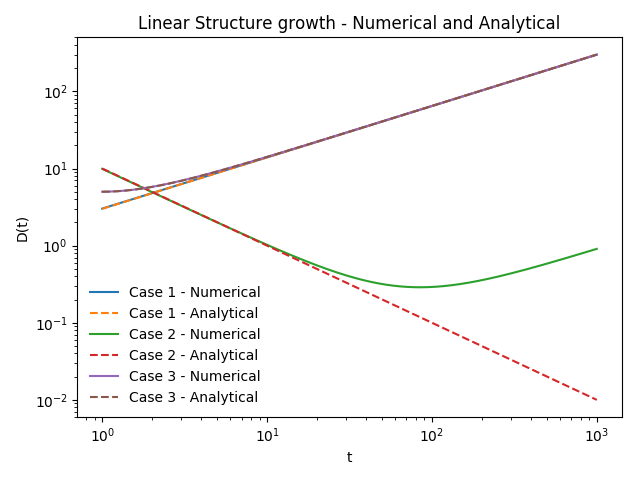
\includegraphics[width=0.8\linewidth]{./plots/3.png}
  \caption{Analytical and numerical solutions to the partial differential equations given in this question.}
  \label{fig:3}
\end{figure}

\subsection{Scripts}

Here we can see the terminal output of the script used for this exercise:
\lstinputlisting{a2_3.txt}

Here is the script used to produce these results: 
\lstinputlisting{a2_3.py}

\section{Zeldovich approximation} 

In this exercise we will be looking at the Zeldovich approximation. 

\subsection{Calculating the linear growth factor to a given redshift.}

Our first task was to integrate the linear growth factor up to a redshift of $z=50$. The integral to be solved is the following:

\begin{equation}
D(z) = \frac{5\Omega_mH_0^2}{2}H(z)\int_z^\infty\frac{1+z'}{H^3(z')}dz'
\end{equation}

Where 

\begin{equation}
H(z)^2 = H^2_0(\Omega_m(1+z)^3+\Omega_\Lambda)
\end{equation}

In order to avoid having to integrate up to $\infty$ we will be substituting $z = \frac{1}{a} -1$. This gives us the following equations:

\begin{equation}
D(a) = \frac{5\Omega_mH_0^2}{2}H(a)\int_0^a\frac{1}{a^3H^3(a')}da'
\end{equation}

Where 

\begin{equation}
H(a)^2 = H^2_0(\frac{\Omega_m}{a^3}+\Omega_\Lambda)
\end{equation}

The resulting value is: $D(1/51) = 0.0196$. The exact number and the way that it was calculated can be found in the print output below. 

\subsection{Calculating the derivative of the linear growth factor at a given redshift}

In order to accomplish this task we had to analytically derive the value of $\dot{D}(t)$. One can calculate this indirectly using the following equation: 

\begin{equation}
\dot{D}(t) = \frac{dD}{da}\dot{a}
\end{equation} 

Where

\begin{equation}
\dot{a} = \frac{H_0}{\sqrt{a}}
\end{equation}


If we use the chain rule we get:

\begin{equation}
\frac{dD}{da} = \frac{5\Omega_mH_0^2}{2}[\frac{dH(a)}{da}I+\frac{dI}{da}H(a)]
\end{equation}

Where

\begin{equation}
I = \int^a_0\frac{1}{a^3H(a)^3}da
\end{equation}


Which gives us: 

\begin{equation}
\dot{D}(a) = \frac{5\Omega_mH_0^3}{2\sqrt{a}}[\frac{-3\Omega_m}{2\sqrt{a^5(\Omega_m+\Omega_\Lambda a^3)}}\int^a_0\frac{1}{a^3H(a)^3}da+\frac{1}{a^3H(a)^3}H_0\sqrt{\frac{\Omega_m}{a^3}+\Omega_\Lambda}]
\end{equation}

The resulting value is: $\dot{D}(1/51) = 1239$ REQUIRE UNITS . The exact number and the way that it was calculated can be found in the print output below. 

\subsection{Evolution of a volume in 2D}

For this exercise we were asked to use the Zeldovich approximation to generate a movie of the evolution of a volume in two dimensions from a scale factor of 0.0025 until a scale factor of 1.0. The movie made for this exercise is called \textit{2D.mp4} and can be found in the directory of this assignment. Besides making the movie we were also asked to plot the position and momentum of the first 10 particles along the $y$-direction vs $a$. These can be seen in Figure \ref{fig:4a} and Figure \ref{fig:4b}. 

\begin{figure}[h!] 
	\begin{center}
    	%
		\subfigure{%
			\label{fig:4a}
			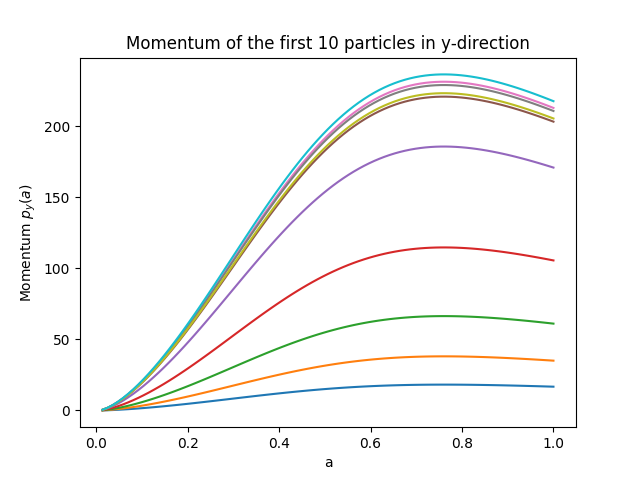
\includegraphics[width=0.45\linewidth]{./plots/4a.png}
		}%
		\subfigure{%
			\label{fig:4b}
			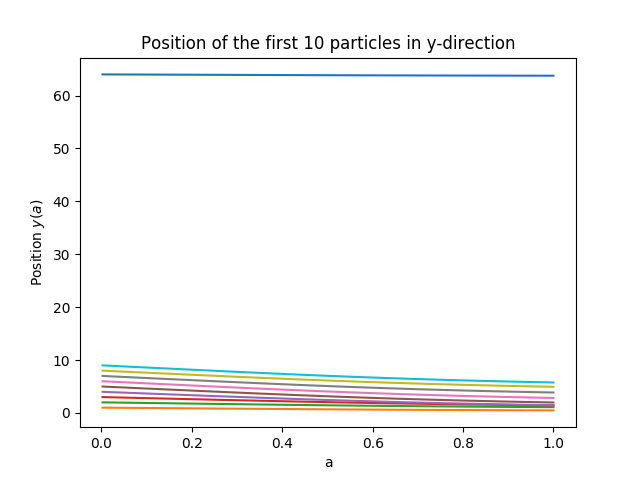
\includegraphics[width=0.45\linewidth]{./plots/4b.png}
		}
	\end{center}
	\captionsetup{width=0.8\linewidth}
	\vspace*{-7mm} %reduce space between caption and figure
	\caption{\textit{Left:} Evolution of the momentum of the first 10 particles (in the y-direction).  \textit{Right:} Evolution of the y-coordinates of these same 10 particles. Note how we see in the right figure that the outer particles (~ 6 through 10) seem to be moving towards the other particles. This is also reflected in the evolution of the momentum which increases much faster for the outer particles and eventually slows down once they reach 'the rest'.}
	\label{fig:4ab}
\end{figure}

\subsection{Evolution of a volume in 3D}

This task was very similar to the previous task except for the fact that we had to make the simulation in 3D. The movies generated for this are named \textit{3D\_ xy.mp4, 3D\_ xz.mp4} and \textit{3D\_ yz.mp4} for each respective slice. We were also asked to plot the position and momentum of the first 10 particles along the $z$-direction vs $a$. 

\begin{figure}[h!] 
	\begin{center}
    	%
		\subfigure{%
			\label{fig:4c}
			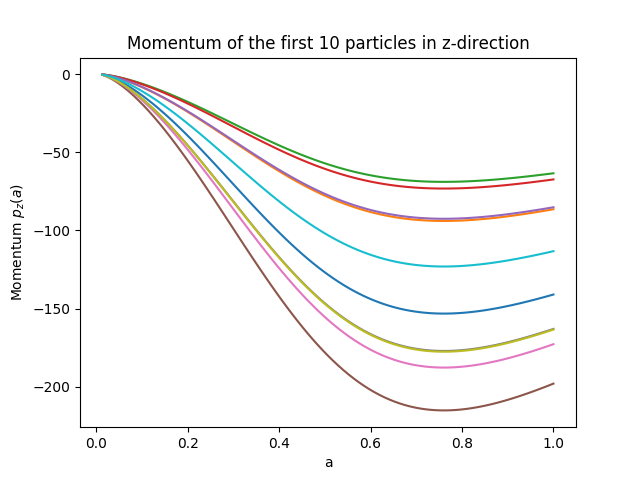
\includegraphics[width=0.45\linewidth]{./plots/4c.png}
		}%
		\subfigure{%
			\label{fig:4d}
			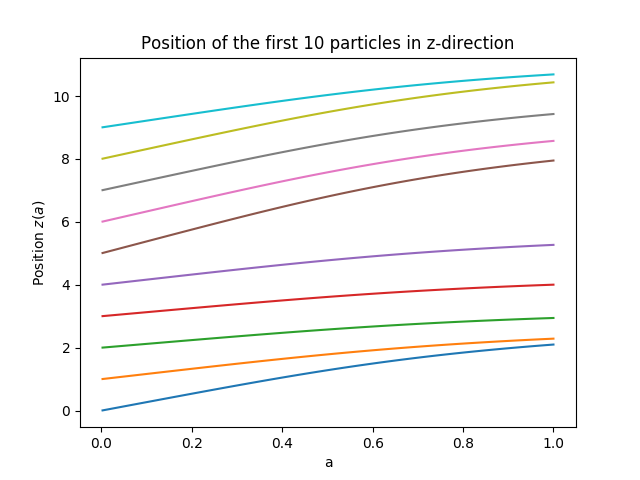
\includegraphics[width=0.45\linewidth]{./plots/4d.png}
		}
	\end{center}
	\captionsetup{width=0.8\linewidth}
	\vspace*{-7mm} %reduce space between caption and figure
	\caption{\textit{Left:} Evolution of the momentum of the first 10 particles (in the z-direction).  \textit{Right:} Evolution of the y-coordinates of these same 10 particles. Similarly to the particles in the previous exercise, the momentum appears to accurately reflect their movement. More displacement in the spacial coordinates implicates a steeper curve in the momentum graph.}
	\label{fig:4ab}
\end{figure}

\subsection{Scripts}

Here we can see the terminal output of the script used for this exercise:
\lstinputlisting{a2_4.txt}

Here is the script used to produce these results: 
\lstinputlisting{a2_4.py}


\section{Mass assignment schemes}

The aim of this assignment was to generate a particle mesh that could be used to calculate a density mesh which could then be used to calculate the gravitational forces in our simulation. 

\subsection{Nearest Gird Point method}

The most simple way to approach this problem is the to add the mass of each particle to the grid point that is closest to it (hence the name 'Nearest Grid Point method'). My 3D implementation of this method generated the mesh visible in Figure \ref{fig:5a}. 

\begin{figure}[h!]
  \centering
  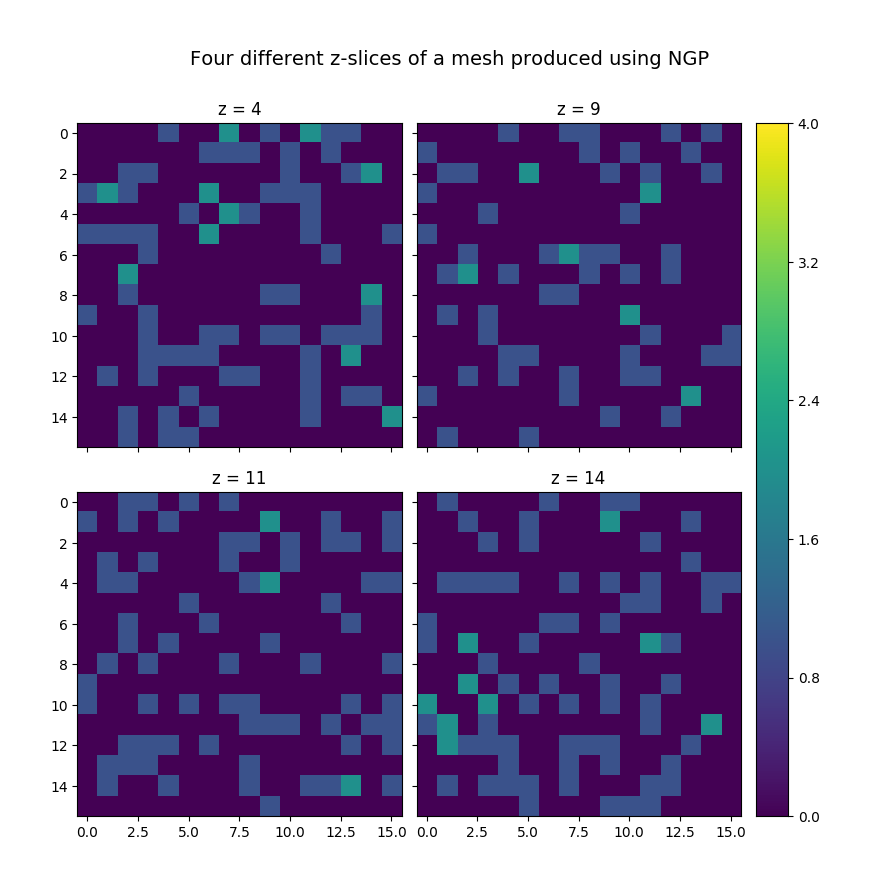
\includegraphics[width=0.7\linewidth]{./plots/5a.png}
  \caption{Four different z-slices of the mesh that was produced using the Nearest Grid Point method.}
  \label{fig:5a}
\end{figure}

\subsection{Testing robustness}

In order to test the robustness of the method we were asked to make a plot of the $x$ position of an individual particle and the value in cell 4 and 0 in 1 dimension (where x varied from the lowest to the highest possible value. In order to accomplish this a 1-D version of the algorithm was coded up (see code below). The resulting graph can be seen in Figure \ref{fig:5b}. 

\begin{figure}[h!]
  \centering
  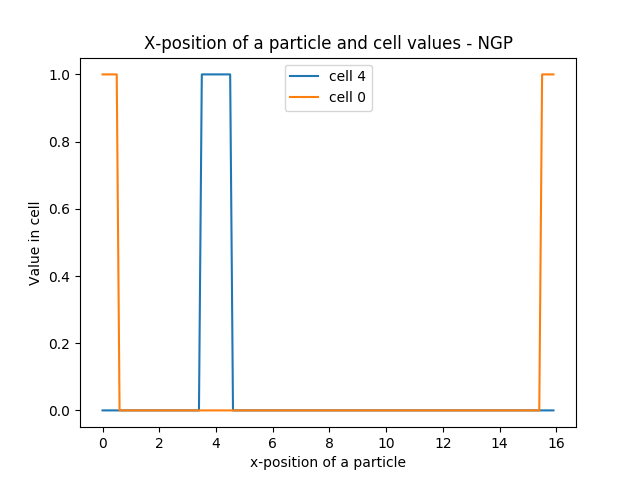
\includegraphics[width=0.7\linewidth]{./plots/5b.png}
  \caption{Here we see the values of cell 4 and cell 0 as a function of the position of a particle along the x-axis. Note how the cell takes on a value of 1 once the particle is within 0.5 cell sizes of it's center. This indicates that the code is working properly.}
  \label{fig:5b}
\end{figure}

\subsection{The Cloud in Cell method}

In the Cloud in Cell method the mass of the particle is distributed among the nearest cells according to how close they are to the particle. The nearer the cell is to a particle, the higher the percentage of the mass assigned to the cell. The implementation of this code can be found below. The z-slices produced using this method may be seen in Figure \ref{fig:5c}. Finally its robustness is assessed using the plot found in Figure \ref{fig:5d}. 

\begin{figure}[h!]
  \centering
  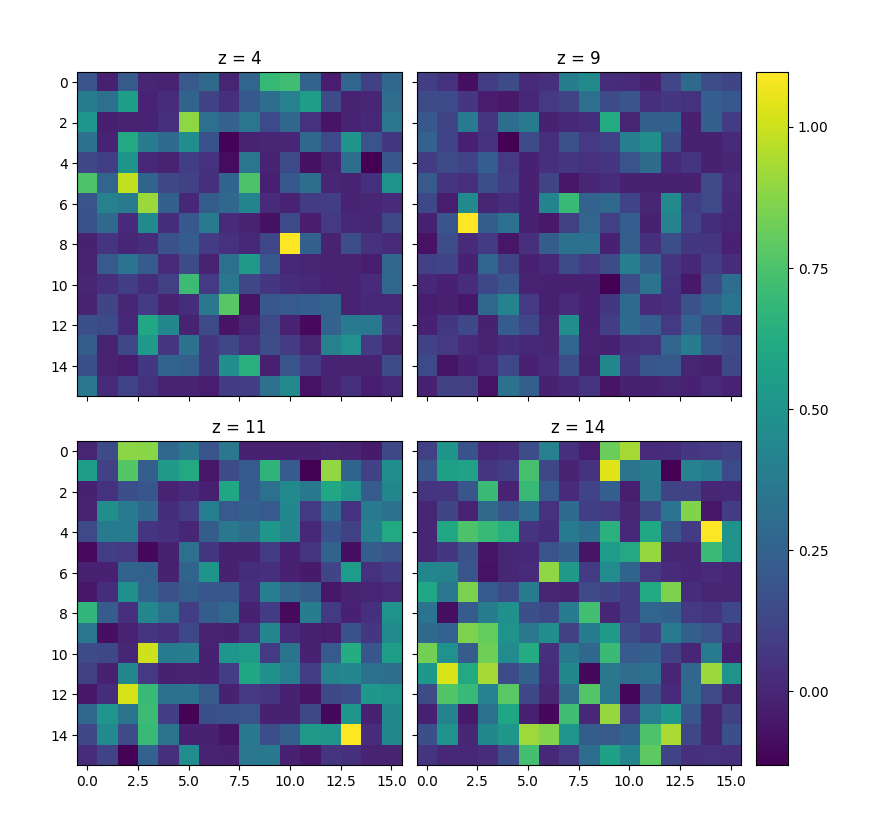
\includegraphics[width=0.7\linewidth]{./plots/5c.png}
  \caption{Four different z-slices of the mesh that was produced using the Cloud in Cell method. Note how the mass in this mesh is far more spread out than in the one produced using the NGP method.}
  \label{fig:5c}
\end{figure}


\begin{figure}[h!]
  \centering
  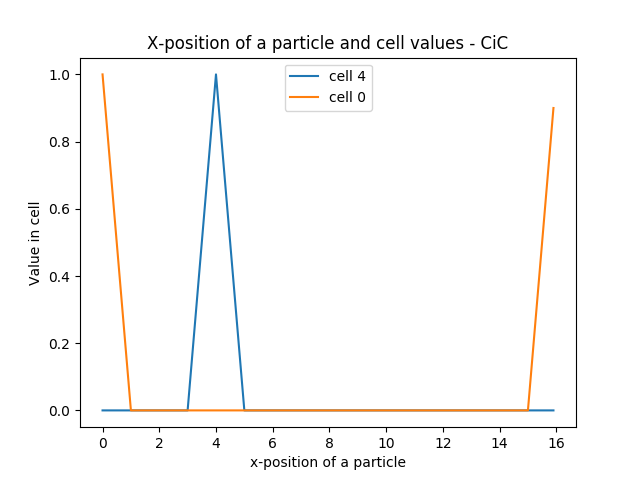
\includegraphics[width=0.7\linewidth]{./plots/5d.png}
  \caption{Here we see the values of cell 4 and cell 0 as a function of the position of a particle along the x-axis. Note how the cells gradually take on more and more of the percentage of the mass of the particle, peaking at 1 when the particle is located at the exact same spot as the cell. After this the value gradually drops back down to 0.  This indicates that the code is working as intended.}
  \label{fig:5d}
\end{figure}

\subsection{1D Fast Fourier Transform Algorithm}

For this exercise the Cooley-Tukey algorithm was used. In Figure \ref{fig:5e} we can see that the 'self-written' algorithm produces the same values as the numpy.fft package and the analytical values. 

\begin{figure}[h!]
  \centering
  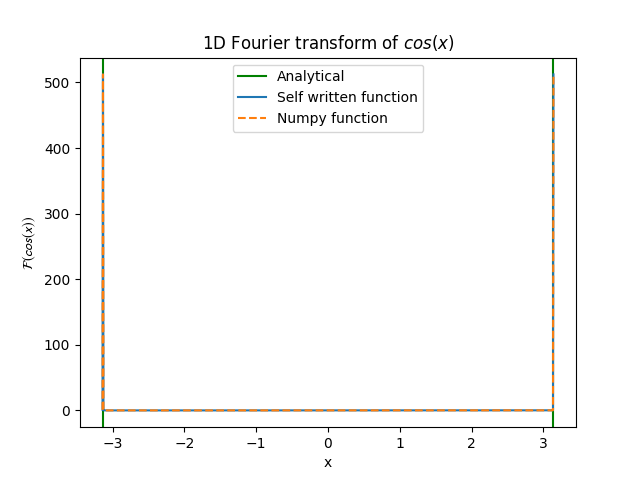
\includegraphics[width=0.7\linewidth]{./plots/5e.png}
  \caption{Plot of the Fourier transform of a $cos(t)$ function as calculated with three different methods. Note how they all appear to give the same values.}
  \label{fig:5e}
\end{figure}

\subsection{2D and 3D Fast Fourier Transform Algorithms}

The next task was to generalize the FFT to 2 and 3 dimensions. The 2D transform was then to be tested by comparing it with the analytical FFT of the same function. These can be seen in Figure \ref{fig:5f}. For the 3D FFT we were to make a plot of a 3D multivariate Gaussian function and plot the 3 slices centered at the center for the three different slice options $x-y, x-z$ and $y-z$. These can be seen in Figure \ref{fig:5g}.

\begin{figure}[h!]
  \centering
  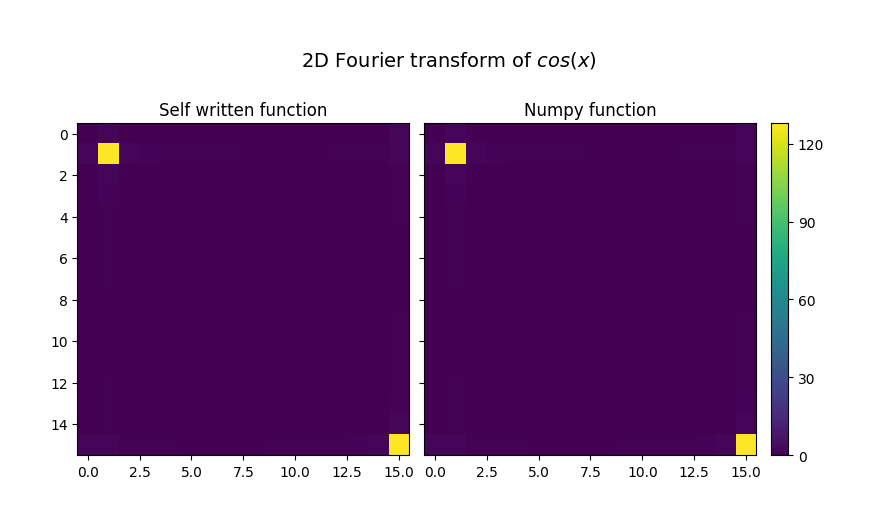
\includegraphics[width=0.7\linewidth]{./plots/5f.png}
  \caption{Plot of the 2D transform.}
  \label{fig:5f}
\end{figure}

\begin{figure}[h!]
  \centering
  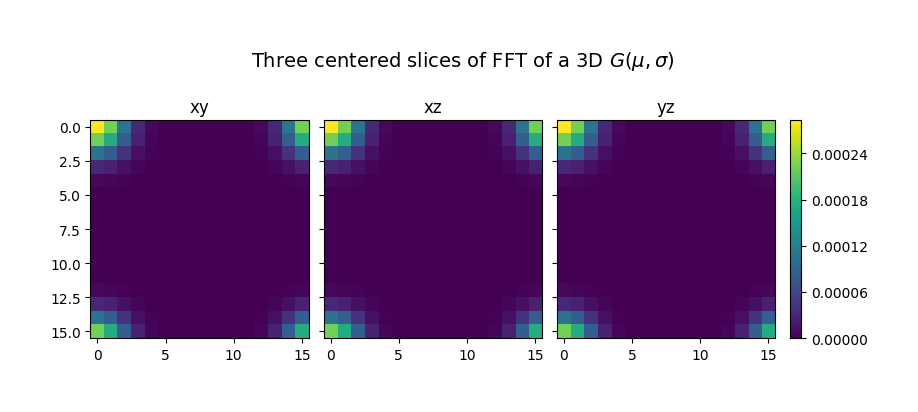
\includegraphics[width=0.7\linewidth]{./plots/5g.png}
  \caption{Slices of the 3D transform of a multivariate Gaussian.}
  \label{fig:5g}
\end{figure}

\subsection{Calculating the potential for the given particles}

For this exercise we were given an equation which we could use to calculate the potential for the given particles. Implementing this required to following thee steps: 

\begin{enumerate}
	\item Taking the Fourier transform of the $\delta$, where $\delta$ is the density distribution (the calculated mesh). 
	\item Dividing the result by $k^2$. 
	\item Applying the inverse Fourier transform.  
\end{enumerate}

The implementation of these steps may be found in the code below. The resulting slices can be seen in Figure \ref{5h} and Figure \ref{5i}. 

\begin{figure}[h!]
  \centering
  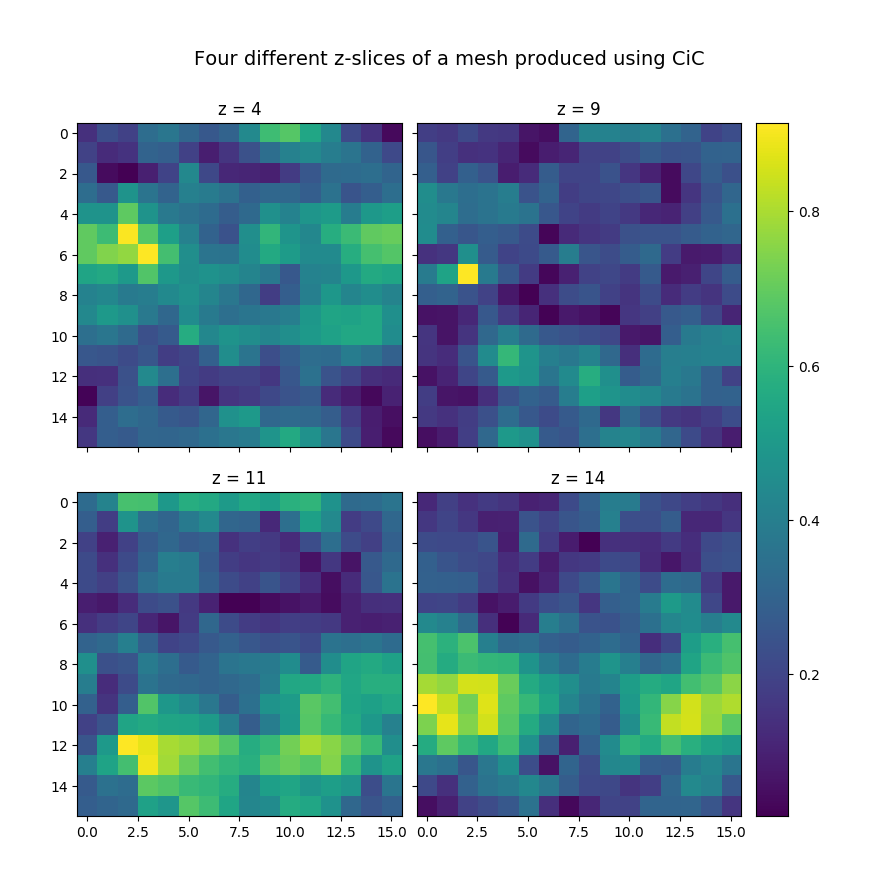
\includegraphics[width=0.7\linewidth]{./plots/5h.png}
  \caption{Plot of the 2D transform of $cos(x,y)$ function.}
  \label{fig:5h}
\end{figure}

\begin{figure}[h!]
  \centering
  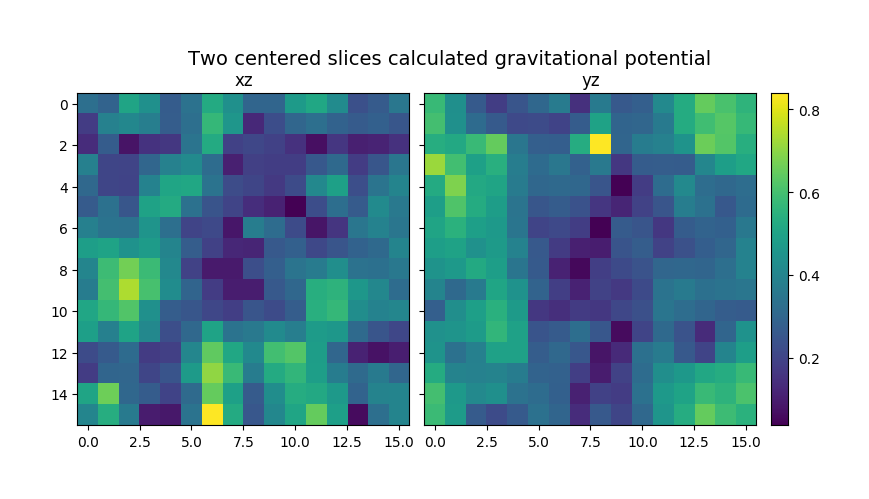
\includegraphics[width=0.7\linewidth]{./plots/5i.png}
  \caption{Slices of the 3D transform of a multivariate Gaussian.}
  \label{fig:5i}
\end{figure}

\subsection{Calculating the potential gradient for the particles}

Now that we had the potential field, we could use it to calculate the gradient of the potential for the first 10 particles. In order to implement this, the gradient was calculated using the central difference method. Afterwards the potential was assigned to the particles using a sort of 'reverse CiC' algorithm. The code can once again be found below as well as the output of the gradients values for the 10 first particles. 

\subsection{Scripts}

Here we can see the terminal output of the script used for this exercise:
\lstinputlisting{a2_5.txt}

Here is the script used to produce these results: 
\lstinputlisting{a2_5.py}

\section{Classifying $\gamma$-ray bursts}

Using the given dataset we were asked to use logistic regression to make a model of the data, using a binary classification for short (0) or long (1) GRB's. 

In order to accomplish this, the data first had to be cleaned up a bit. We threw out all the rows that were not classified as GRB's in the first place. We dealt with the missing data by simply setting those values to 0 (instead of -1). The time (T90) was used in order to produce the labels for the data, but was also thrown out once this was done. The remaining data was then split up into a training and a test set (80\% and 20\% respectively). In Figure \ref{fig:6} we can see the results. After 4000 epochs we reached an accuracy of $69.3\%$ on the training set, $70.5\%$ on the test set and $69.5\%$ on the entire data set. Training for more epochs would result in a drop of accuracy in the test set, meaning that the models was probably over fitting at that point.  

\begin{figure}[h!]
  \centering
  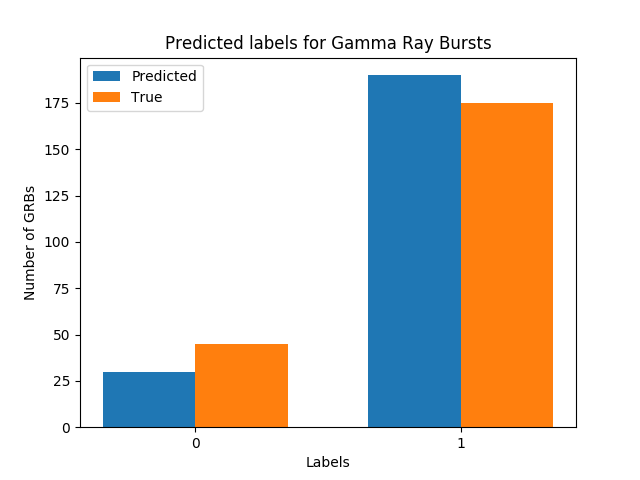
\includegraphics[width=0.7\linewidth]{./plots/6.png}
  \caption{These are the results of the classifier after 4000 training epochs. Label 0 represents the short bursts while 1 represents the long bursts.}
  \label{fig:6}
\end{figure}

\subsection{Scripts}

Here we can see the terminal output of the script used for this exercise:
\lstinputlisting{a2_6.txt}

Here is the script used to produce these results: 
\lstinputlisting{a2_6.py}

\section{Building a quadtree}

For this exercise our goal was to build a Barnes-Hut quadtree with at most 12 particles per leaf node. When writing the code for this exercise I based my class object structure on the one used in this online example: \textit{https://kpully.github.io/Quadtrees/}. The particles and their corresponding nodes are plotted in Figure \ref{fig:7}.

\begin{figure}[h!]
  \centering
  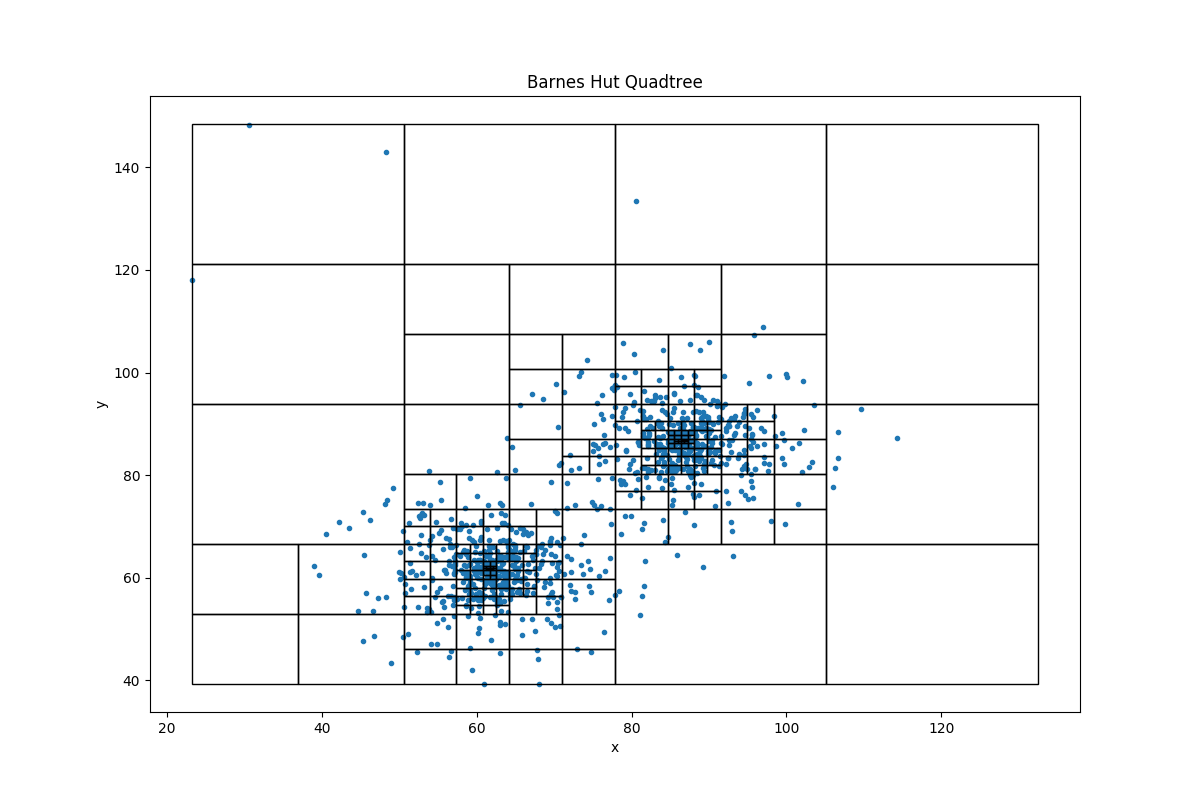
\includegraphics[width=0.8\linewidth]{./plots/7.png}
  \caption{In this figure we can see the Barnes Hut Quadtree built for the given dataset.}
  \label{fig:7}
\end{figure}

\subsection{Scripts}

Here we can see the terminal output of the script used for this exercise:
\lstinputlisting{a2_7.txt}

Here is the script used to produce these results: 
\lstinputlisting{a2_7.py}

\end{document}


 

